%!TEX root =  main.tex
%!TEX encoding = UTF-8 Unicode
\chapter{協調フィルタリング:モデルベース法}
\label{chap:modelbase}
\indexmain{モデルベース法}\indexmain{model-based method}

モデルベース法では,活動利用者に推薦をする前にモデルを構築する.
ノーフリーランチ定理により万能な予測モデルは存在しないので,多様なモデルが目的に合わせて提案されている.これらを順次紹介する.

\section{クラスタモデル}
\label{sec:clustermodel}

嗜好パターンが類似している利用者が好むものを推薦するという手順を,直観的に実装したのがクラスタモデルである\cite{uai:98:01,epublist:039}.
クラスタとは対象の集合を分割した部分集合で,同じクラスタ内の対象は互いに似ているが,違うクラスタでは似ていないという条件を満たすものである.
こうしたクラスタを得る手法をクラスタリングという\cite{jpublist:034,jb:038:00,jb:020:00}.
この手法を用いて,嗜好パターンが類似している利用者のクラスタに,標本利用者の集合を分割する.
ここで,利用者間の類似度は,\ref{chap:memorybase}章の式\eqref{eq:glsim}のPearson相関係数のように,いろいろなアイテムへの評価値がどれくらい類似しているかによって測る.
活動利用者への推薦は,活動利用者と各クラスタとの類似度を調べ,最も似ているクラスタを見つける.
そして,そのクラスタ中の標本利用者の平均評価値が高いアイテムから順に活動利用者に推薦する.
この方法には,利用者集合とアイテム集合を同時に分割する共クラスタリング(co-clustering)を使う改良\cite{icdm:05:05}などがある.

このモデルでは,利用者DBを何個のクラスタに分けたかによって,推薦の質が大きく変わる.
クラスタ数を小さく設定すると,おおまかであまり個人化されていない推薦がなされる.そのため,cold-start問題に対して比較的強い.
しかし,推薦パターンの種類はたかだかクラスタ数に制限されるので,多数の嗜好データを集めても,ある程度以上に個人化された推薦はできない.
一方,クラスタ数を多くすると,スタートアップ問題\index{スタートアップ問題}\index{start-up problem}に対して弱くなるが,推薦の個人化の度合いは高まる.
また,クラスタ数が多すぎると安定したクラスタを求めるのが難しくなる問題もある.
よって目的に合わせてクラスタ数を調整する必要がある.

この方法には,実現が直観的なことに加え,モデルの構築も比較的高速であり,単純なので実装も容易であるといった利点がある.
推薦時も,各クラスタと活動利用者の類似性を調べるだけなので,計算量はクラスタ数だけに比例し,高速である.
欠点としては\term{灰色の羊問題}{gray sheep problem}~\cite{ej:048}がある.
例えば,映画の推薦を考えた場合,特定のジャンルのものだけを鑑賞する利用者はむしろ少なく,サスペンスとホラーなど複数のジャンルの映画を見るであろう.
クラスタモデルでは,利用者を特定のクラスタに分けてしまうため,こうした白でも黒でもない灰色の羊の利用者に適切な推薦ができない.
%こうした灰色の羊問題を生じない,あるアイテムが好きなら,他のアイテムはあまり好まない排他的な性質がある分野に適応すべきだろう.

\section{関数モデル}
\label{sec:funcmodel}

利用者が好きなものほど大きな値をとる効用関数(utility function)や,評価値そのものを予測する関数を用いるモデルを,本稿ではまとめて関数モデルと呼ぶ.
そして,これらのモデルの獲得を,回帰問題,クラス分類問題,および順序回帰問題に帰着させて解く.これらの手法を順次紹介する.

\subsection{回帰問題に帰着させる方法}

最初に,回帰問題に帰着させる手法から紹介する.
最も簡単な線形関数の場合を考える.
\ref{sec:item-item}節の式\eqref{eq:iicf}は,詳細を無視すれば次のような線形モデルとみなせる.
\begin{equation}
\hat{r}_{ay} = \sum_j w_{yj} r_{aj}
\label{eq:itemlinear}
\end{equation}
\ref{sec:item-item}節では,パラメータ$w_{yj}$はアイテム$y$と$j$の嗜好パターンの類似性を,相関係数など経験的に選んだ類似度で決めた.
しかし,与えられた評価値の集合を訓練事例として,機械学習の手法を適用すれば,もっと予測精度の高い関数を獲得できるのではないか?
この考えに従い,これらのパラメータを決める問題を\term{回帰}{regression}や\term{あてはめ}{fitting}~\cite{eb:053:00,jpublist:077x}という機械学習や統計的予測の問題に帰着させ解く.

まず,回帰モデルを,評価値行列$\bfR$行列の分解として捉えてみよう.
与えられた行列$\bfR$の未評価アイテムの部分は欠損しているが,欠損していない完全な評価値行列$\bfR^\ast$を考え,この行列を次のように分解する.
\begin{equation}
\bfR^\ast\approx \bfU^\T\bfV
\label{eq:factormodel}
\end{equation}
ここで,$\bfU$と$\bfV$の大きさは,それぞれ$K\times n$と$K\times m$である.
$\bfU$の第$x$列ベクトル$\bfu_x$は利用者$x$の特徴を,$\bfU$の第$y$列ベクトル$\bfu_y$はアイテム$y$の特徴を表している.
すると,利用者$x$へのアイテム$y$への評価値は$r^\ast_{xy} \approx \bfu_x^\T \bfv_y$のようなモデルで表される.
$\bfu_x$の要素を説明変数と,$\bfv_y$の要素をパラメータとみなせば式\eqref{eq:itemlinear}と同等のモデルであり,逆に$\bfv_y$を説明変数にすれば,式\eqref{eq:glscr}と類似したモデルとも解釈できる.
ここでもし$K$が$\max\{m,n\}$なら,近似ではなく厳密に$\bfR^{\ast}=\bfU^\T\bfV$となるように分解できる.
だがこれでは,観測データを書き写しただけで,嗜好パターンを要約したモデルとはいえない.
また,実際に観測できる評価値行列は$\bfR^\ast$ではなく,欠損のある$\bfR$である.
そこで,$K$を$K\ll m,n$に固定し,$\bfR^\ast$との期待的な損失を最小化するように,$\bfR$を$\bfU$と$\bfV$に分解することで,モデルを獲得する.

こうした分解をするには,\term{行列分解}{matrix decomposition}の手法を用いる.
こうした手法の一つ\cite{sigir:02:01}を述べる.
%式\eqref{eq:iicf}は$m$個のアイテムへの評価で利用者を表現した
%が,因子分析では$K$個の因子(factor)で利用者を表す.
%すなわち,映画の場合であれば,個々の作品への評価ではなく,ヒュー
%マンドラマが好きだとか,ある女優が出ているといやだといった,より一
%般的な因子で利用者が記述されているようなものである.
%すると,式\eqref{eq:factormodel}で,$X$の列ベクトルは$K$個の因子で
%記述した利用者を,$Y$の列ベクトルはアイテムの$K$個の因子への関連性
%を表したものと解釈できる.
この方法では,残差$\prn{\bfR-\bfU^\T\bfV}$の各要素が正規分布に従うとしてモデル化し,観測された評価値の生成確率が高くなるように$\bfU$と$\bfV$を計算する.
この行列分解手法を\term{因子分析}{factor analysis}という.
分解ができれば,任意の利用者の任意アイテムに対する推定評価値$\hat{r}_{xy}=\bfu_x^\T \bfv_y$が計算できる.
しかし,実際の$\bfR$には欠損値があるので,文献\cite{sigir:02:01}では,これらの欠損値を潜在変数とみなしてEMアルゴリズム\cite{jrss:77:01}\index{EMアルゴリズム}\index{EM algorithm}を適用して解いている.
欠損値に対処する方法は,潜在変数以外にも,全員が必ず評価するアイテム集合を利用する,欠損値を平均値などで補完する,欠損した要素は無視して損失を計算する\cite{kdd:07:01}といった方法もある.
回帰モデルは単純なので,演算操作が複雑になるプライバシー保護協調フィルタリング(\ref{chap:privacy}章)などへの適用や,カーネルを使った非線形回帰を導入して予測の向上を図るといった拡張が可能である.

次に文献\cite{kdd:99:04}の\textbf{Horting}\index{Horting}法を紹介する.
式\eqref{eq:itemlinear}のように全体を一つの線形モデルで表すと,大まかすぎて予測精度が低くなる場合がある.
そこで,嗜好が類似している利用者の間で局所的に線形モデルを構築する.
利用者$a$について,共通に評価したアイテムが十分に多い利用者$x$を見つける.
さらに,これらの利用者$x$の評価値$r_{xy}$から$\hat{r}_{ay}=\theta_{ax}r_{xy} + b_{ax}$の線形関数で,利用者$a$のスコアを高精度で予測できる利用者を選び出す.
このとき,利用者$x$は利用者$a$を予測可能といいう.
なお,$\theta_{ax}$や$b_{ax}$は,両者が共通に評価しているアイテムの評価値から計算可能である.
次に,利用者をノードとし,$x$から$a$への予測可能性を逆向きの$a$から$x$への有向辺でを示すグラフを生成しておく.
このグラフを用いて,利用者$a$のアイテム$y$への評価値を推定する.
利用者$a$から直接リンクしている利用者で,アイテム$y$を評価している利用者の集合を$\calX'_y$とする.
この集合が空でなければ,アイテム$y$への予測評価値は,$\calX'_y$中の利用者それぞれによる予測評価値の平均とする.
\[
 \hat{r}_{ay}=\frac{1}{|\calX'_y|}
\sum_{x\in\calX'_y}\theta_{ax}r_{xy} + b_{ax}
\]
もし,$\calX'_y$が空なら,リンクを2段たどり,アイテム$y$を評価している利用者集合を求め$\calX''_y$とする.この集合が
空でなければ次式で予測評価値を求める.
\[
\textstyle
 \hat{r}_{ay}=\frac{1}{|{\calX''}_y|}\sum_{x\in\calX''_y}\theta_{ax'}(\theta_{x'x}r_{xy} + b_{x'x}) + b_{ax'} 
\]
ただし,$x'$は,各$x$について$x$と$a$を中継する利用者である.
さらに$\calX''_y$も空ならば,3段以上のリンクを考慮する.

\subsection{クラス分類問題に帰着させる方法}

回帰と並ぶ代表的な機械学習の枠組みである\term{クラス分類}{classification}も利用できる.
アイテム$y$への評価値$r_{ax}$は,$\calR$中の値の一つをとるので,その大小関係を無視すれば,クラスと考えることができる.
また,分類するアイテム$y$の特徴量には,このアイテムへの他の利用者による評価値や,活動利用者の他のアイテムへの評価値が利用できる.
あとは,これらの特徴量で表されたアイテムが分類されるべきクラス,すなわち評価値を予測するモデルをクラス分類の学習手法によって獲得すればよい.

このような方法として,\term{逐次型二項関係学習法}{Cross-G-Learn-Relation method}\cite{icml:98:01,jb:032:04}を紹介する.
なお,原論文では評価大小関係を考慮する工夫がさらになされているが,ここでは簡潔に記す.
これは,各クラスごとに,対象の分類されやすさを表す関数を獲得し,その関数の値が最大になるクラスに対象を分類する.
利用者$x$のアイテム$y$の評価値を予測するとき,逐次型二項関係学習法では,アイテム$y$への他の利用者の評価と,利用者$x$のその他のアイテムへの評価を入力とした次の関数を用いる
\begin{equation}
\hat{r}_{xy}=\arg\max_{r\in \calR}
\prn{\sum_{i\st r_{iy}=r}v_{xi}+\sum_{j\st r_{xj}=r}w_{yj}}
\label{eq:cglr}
\end{equation}
利用者$x$が仮にアイテム$y$の評価値を$r$としたとき,
第1項ではアイテム$y$についての評価が同じ$r$である利用者$i$について,利用者間重み$v_{xi}$の総和を求める.
同様に,第2項では利用者$x$が同じ$r$と評価をしているアイテム$j$について,アイテム間重み$w_{yj}$の総和を求める.
すなわち,類似利用者と類似アイテムの評価値の両方を考慮している.
重み$v_{xi}$と$w_{yj}$は\term{オンライン学習}{online learning}\cite{jjsai:99:02}の枠組みで求める.
これは,行列$\bfR$の形式で評価値がまとめて与えられてから学習するのではなく,誰かが何かアイテムを評価して,$r_{xy}$が一つ与えられるごとに重みをより適切なものに更新する方法である.
各評価値を与えられるごとに,予測値とその与えられた値とを比較することを繰り返し,ある時点までの累積の誤りを小さくするようにモデルを学習する.
もう少し詳しく述べると,最初に全ての重み$v_{xi}$と$w_{yj}$を初期化する.
その後,$r_{xy}$が観測されるたびに,利用者$x$以外でアイテム$y$を評価済みの全ての利用者$i$について,$r_{xy}=r_{iy}$なら重み$v_{xi}$を増やし,そうでないなら減らす.
さらに,利用者$x$が評価している$y$以外の全てのアイテム$j$について,評価値が一致すればやはり重み$w_{yj}$を増やし,そうでなければ減らす.
このように評価値が与えられるごとに重みを更新する.
この方法はオンライン学習なので,モデルベースだが,アイテムや利用者が追加されても対応できる特徴がある.
ただし,アイテムや利用者の削除には対応できない.

\subsection{順序回帰問題に帰着させる方法}

\ref{sec:explicitrating}節では,採点法や格付け法による評価値は,本来は順序付カテゴリとして扱うべきものであることを述べた.
すなわち,評価値が2のアイテムは,4のアイテムの半分程度好きなのではなく,評価値3のアイテムより,4のアイテムの方がより好きであるということだけを示している.
こうした順序付カテゴリ値を予測する問題は順序回帰と呼ばれる.
この順序回帰を,ブースティング (boosting) \cite{icml:96:02,jjsai:99:01} の枠組みで扱う\textbf{RankBoost}~\cite{icml:98:03,jmlr:03:02} \index{rankboost@RankBoost}で推薦をする研究などがある.
後に,この順序回帰を用いた,内容ベースと協調フィルタリングのハイブリッド法を\ref{sec:combmethod}節で紹介する.

\section{確率モデル}
\label{sec:probmodel}

モデル化に用いた関数が確率分布として解釈できるものを本稿では特に確率モデルと呼ぶ.
これら確率モデルを,大きく履歴条件型と共起型の二つに分け,順に説明する.

\subsection{履歴条件型}

履歴条件型の確率モデルでは,活動利用者のアイテム$j$への評価値を次の条件付期待値で予測する\cite{uai:98:01}.
\begin{align}
\hat{r}_{ay} & = \expect\bra{r_{ay}|r_{aj}\st j\in\calY_a}\nonumber\\
& = \sum_{r\in\calR} r\;\pb{r_{ay}=r|r_{aj}\st j\in\calY_a}
\label{eq:escoreg}
\end{align}
これは,活動利用者の過去の嗜好データが与えられたときの,活動利用者のアイテム$y$への評価値の条件付期待値である.
実際には,式\eqref{eq:escoreg}中の確率分布は未知なので,推定した関数を利用する.
式中では他の標本利用者の嗜好データが参照されていないが,確率分布の推定の過程で,これらの嗜好データを利用するため,協調フィルタリングによる推薦といえる.
また,適合/不適合の2値の嗜好データ,すなわち$\calR=\cbr{0,1}$の場合,式
\eqref{eq:escoreg}は単なる条件付確率分布となる.
\begin{equation}
\hat{r}_{ay}=\pb{r_{ay}=1|s_{aj}\st j\in \calY_a}
\label{eq:escore}
\end{equation}
このように簡潔になるので,予測評価値を提示する評価閲覧よりも,適合か不適合かの判定ができればよい適合アイテム発見タスクに適す.
\index{適合アイテム発見}\index{finding some good items}
この履歴条件型モデルでは,条件付確率\eqref{eq:escore}の計算のため,肯定的評価の$r_{xy}=1$と否定的評価の$r_{xy}=0$の両方の場合の訓練事例が必要である.
しかし,\ref{chap:input}章で述べたように,暗黙的な評価では,購入や閲覧などの行動がなかったことで否定的な評価とみなす.
すると,未評価と否定的評価は混同され,$r_{xy}=0$となる事例にはノイズが多くなる.
そのため,未評価と否定的評価が明確に区別される事例が必要となり,この履歴条件型ではこうした暗黙的評価では不利になる.

式\eqref{eq:escoreg}中の条件付確率は,$\calY_a$に依存するため,各利用者について個々にモデルを獲得する必要が生じ,実用的ではない.
そこで実際には,利用者には依存しない,次の全アイテムへの評価の同時分布を求める.
\begin{equation}
\Pr[r_{\cdot y}\st y\in \calY]
\label{eq:jprob}
\end{equation}
そして,式\eqref{eq:escoreg}中の条件付分布は,ベイズ則と不要な変数を周辺化で消去することで計算する.
だが,各$r_{\cdot y}$は$|\calR|$個の値をとることが可能で$|\calY|=m$なので,この分布の定義域は$\calR^{\calY}=\calR_{1}\times\calR_{2}\times\dotsb\times\calR_{m}$である.
よって,この分布の飽和モデルのパラメータ数は$|\mathcal{R}|^m-1$となり,$m$に対して指数的に増加する.
しかし,データは疎で$m$は大きいので,単純に評価値の各組み合わせの頻度を数え上げて,この飽和モデルのパラメータを推定することは現実的ではない.
そこで,このような場合の一般的な対策を導入し,変数$r_{\cdot y}$の間に部分的な条件付独立性を仮定し学習すべきパラメータ数を減らす.
このような条件付独立性を導入した確率モデルを,依存関係をグラフで表現して示すため,一般にグラフィカルモデルという.
\index{グラフィカルモデル}\index{graphical model}
その一つである\term{ベイジアンネットワーク}{Bayesian network}\cite{jb:037:00}は\cite{uai:98:01}で利用されている.
ベイジアンネット全般の問題として独立性の構造をうまく設計する難しさがあるが,うまく設計できれば学習も,推薦も効率的に実行できる.
また,式\eqref{eq:escoreg}の条件付確率を直接内部構造としてもつ確率モデルである\textbf{依存性ネットワーク (dependency network) }を使う\cite{jmlr:00:01}などもある.
このモデルでは,同時確率から条件付確率へ変換が不要なので,実行時の推薦は高速に実行できるが,事前のモデル学習の計算量は増える.

\subsection{共起型}

もう一方の共起型の確率モデルについて述べる.
このモデルでは,ある利用者が,あるアイテムを評価したことを,その利用者が$x$であるという事象と,そのアイテムが$y$であるという事象が共起しているととらえる.
そして,この共起確率をモデル化する.
このモデル化には,自然言語処理で文書と語の共起確率を表すために考案された\textbf{確率的潜在意味解析 (probabilistic latent semantic analysis; pLSA)}~\cite{uai:99:01}\indexmain{pLSA}を利用する.
この確率モデルは非常に柔軟で,純粋な協調フィルタリングだけでなく,評価の揺らぎ,アイテムの情報,コンテキスト情報,および個人属性情報などの要因を導入するといった拡張が可能である.

本節では,利用者の嗜好データのみに基づく協調フィルタリングを対象としたモデル\cite{ijcai:99:01}を紹介する.
最初に,利用者とアイテムの共起関係だけを使うモデルについて述べる.
利用者とアイテムに対し,それぞれ$\calX=\cbr{1,\dotsc,n}$と$\calY=\cbr{1,\dotsc,m}$中のいずれかの値を取る多値の確率変数$X$と$Y$を割り当てる.
嗜好データを,利用者$x$がアイテム$y$を購入するという行為で暗黙的に獲得する場合を考える.
これは,$X=x$という事象と,$Y=y$という事象が共起していることに相当する.
また,$\calR=\cbr{0,1}$であるとき,$r_{xy}=1$となる対$(x,y)$が観測されることとも等価である.
履歴条件型の確率モデルでは$r_{xy}=0$となる事例も必要であったが,共起型では$r_{xy}=1$となる事例だけでモデルが学習できる.
このため,未評価と不支持が区別できない暗黙的評価の場合に,この共起型確率モデルは便利である.

さらに,このモデルで重要な役割をはたす\term{潜在変数}{latent variable} $Z$(\textbf{隠れ変数 (hidden variable)} ともいう)を導入する.
これも多値変数で$\calZ=\cbr{1,\dotsc,K}$中の値をとり,潜在的な嗜好のパターンを表す.
この潜在変数の値はデータとして観測されることはなく,モデルの中でのみその存在を仮定する.
これはクラスタモデルと類似しているので,灰色の羊問題(\ref{sec:clustermodel}節)\index{灰色の羊問題}\index{gray sheep problem}が生じるように思える.
だが,$K$個のパターンのうちどれか一つに割り当てるのではなく,それらが混ざり合った状態を考慮するので,この問題は生じない.
そして,この潜在変数を用いて,$x$と$y$の同時確率を,次式で表すのがpLSAモデルである.
\begin{align}
 \pb{x,y}& = \sum_{z\in \calZ}\pb{x}\pb{z|x}\pb{y|z}\label{eq:origplsamodel}\\
& = \sum_{z\in \calZ}\pb{x|z}\pb{y|z}\pb{z}
\label{eq:plsamodel}
\end{align}
このモデルでは,$z$が与えられたときに$x$と$y$が条件付独立であることを仮定して,モデルのパラメータの総数を減らしている.
また,$\pb{x|z}$,$\pb{y|z}$,$\pb{z}$はそれぞれカテゴリ分布に従う.

\begin{figure}
\centering
\subcaptionbox{評価値なし\label{fig:latentmodel:a}}%
{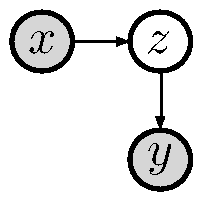
\includegraphics[width=0.3\linewidth]{plsa.pdf}}%
\hspace{0.1\fullwidth}%
\subcaptionbox{評価値あり\label{fig:latentmodel:b}}%
{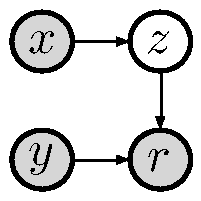
\includegraphics[width=0.3\textwidth]{plsa2.pdf}}
\caption{pLSAモデル\cite{ijcai:99:01}}
\label{fig:latentmodel}
\end{figure}

図\ref{fig:latentmodel:a}は,\termmain{グラフィカルモデル}{graphical model} という表現方法でpLSAモデルを図示したものである.
このグラフで,灰色のノードは値が観測される$X$や$Y$のような\term{観測変数}{observed variable}(\textbf{可視変数 (visible variable)} ともいう)を,白いノードはその値が観測されない潜在変数を表す.
有向辺は確率的な依存関係を表し,辺が出ている変数に,辺が入っている変数が依存することを表す.
また,この図にはないが,値が確定しているパラメータは黒い点で表し,同じ確率変数を複数回サンプリングすることを示すプレートという表現もある.
これらの表現については教科書\cite[8章]{jpublist:077x}などを参考にされたい.

モデルのパラメータは$\bfTheta = \prn{\cbr{\pb{x|z}}, \cbr{\pb{y|z}},\cbr{\pb{z}}}$であるが,これらを最尤推定で求める.
すなわち,いろいろな利用者がいろいろなアイテムを評価した,$N$個のデータ$\calD=\cbr{(x_i,y_i)}_{i=1}^N$に対する次の対数尤度を最大にするように求める.
\[
\pb{\calD; \bfTheta} = \sum_{(x,y)\in \calD} \ln\pb{X=x, Y=y; \bfTheta}
\]
潜在変数があるため,この最尤推定は\termmain{EMアルゴリズム}{EM algorithm}\cite{jrss:77:01,jpublist:077x}によって行う.
具体的には次の二つのステップを交互に反復する.
一つ目のEステップでは,パラメータ$\cbr{\pb{z|x}},\cbr{\pb{y|z}},\cbr{\pb{z}}$が与えられたときの,潜在変数
の分布を求める.
\begin{equation}
\pb{z|x,y}=\frac{\pb{z}\pb{x|z}\pb{y|z}}{\sum_{z'}\pb{z'}\pb{x|z'}\pb{y|z'}}
\label{eq:estep}
\end{equation}
二つ目のMステップでは,前のステップで求めた分布$\pb{z|x,y}$を用いてパラメータを更新する.
\begin{align}
\pb{x|z} & = \frac{\sum_y n\prn{x,y} \pb{z|x,y}}{\sum_{x',y}n(x',y)\pb{z|x',y}}\label{eq:mstepx}\\
\pb{y|z} & = \frac{\sum_x n(x,y) \pb{z|x,y}}{\sum_{x,y'} n(x,y') \pb{z|x,y'}}\label{eq:mstepy}\\
\pb{z} &=\frac{\sum_{x,y}n(x,y)\pb{z|x,y}}{N}\label{eq:mstepz}
\end{align}
ただし,$n(x,y)$は,$x$と$y$が共起している$\calD$中の対の数である.
以上の手続きを収束するまで反復すると,パラメータが計算できる.
そして,次式の$\pb{y|x}$を求めておき,
\begin{equation}
\pb{y|x} = \frac{\sum_z\pb{x|z} \pb{y|z} \pb{z}}{\sum_{y',z}\pb{x|z} \pb{y'|z} \pb{z}}
\end{equation}
活動利用者$a$がアイテム$y$を好む度合いは$\pb{Y=yj|X=a}$の大きさで測る.
活動利用者$a$に対しては,この度合いを最大化する次のアイテム$y^\ast$を推薦すればよい.
\begin{equation}
y^\ast=\arg\max_{y\in\cbr{\calY\backslash\calY_{a}}}\Pr[Y=y|X=a]
\end{equation}
なおpLSAでは訓練データ中に現れない利用者,すなわち,$a\notin\calX$の場合にはこの方法では推薦できない.
このような新規利用者を扱うことを情報検索の文脈ではfolding-in\index{folding-in}という.
このfolding-inを行う方法として,潜在変数とアイテムしか現れないパラメータはそのまま固定し,利用者が関連するパラメータ$\pb{x|z}$のみを更新する手続きが提案されている\cite{misc:089}.

次に,利用者$X$とアイテム$Y$に,評価値を表す確率変数$R$も加えた拡張を考える.
この変数は,評価値の値域$\calR$中の値をとる多値変数である.
このモデル化では$X=x$,$Y=y$,および$R=r$の共起確率$\pb{x,y,r}$を扱う.
そして,利用者$a$のアイテム$y$の推定評価値$\hat{r}_{xy}$は最頻値
\[
\hat{r}_{xy}=\arg\max_{r\in\calR}\Pr[R=r|X=a,Y=y]
\]
や期待値
\[
\hat{r}_{xy}=\frac{1}{\abs{\calR}}\sum_{r\in\calR}r\;\pb{R=r|X=a,Y=y}
\]
で計算する.なお,$\pb{r|x,y}$は$\pb{x,y,r}$から計算できる.
図\ref{fig:latentmodel:b}は$\Pr[x,y,r]$のモデル化の一例である.
このモデルでは,利用者$x$は$z$で表されるグループに分類され,そのグループ$z$とアイテム$y$に依存して評価値$r$が決まると解釈できる.
モデルを決めれば,あとは対数尤度を最大化するパラメータをEMアルゴリズムで求めればよい.
文献\cite{ijcai:99:01}では他にもいくつかのモデルを挙げている.
これらのモデルは評価値を離散変数で表し,カテゴリ分布に従うと考えているので,評価値の大小関係を無視している.
そこで離散の評価値を実数値として扱うことで大小関係を考慮し,それがガウス分布に従うとするモデルもある\cite{sigir:03:01}.
どのモデルが適切かだが,一般には\ref{sec:recomtype}節で述べた交差確認法で,予測精度を最大にするようなものを選ぶ.

\begin{figure}
\centering
\subcaptionbox{decoupled\label{fig:decoupledmodel:a}}%
{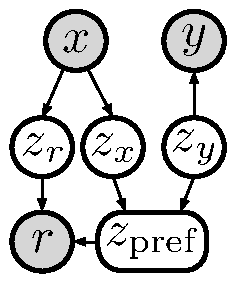
\includegraphics[width=0.3\textwidth]{decoupled.pdf}}
\hspace{0.1\fullwidth}%
\subcaptionbox{preferred ordering\label{fig:decoupledmodel:b}}%
{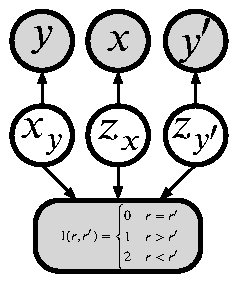
\includegraphics[width=0.3\textwidth]{preford.pdf}}
\caption{評価値の揺らぎを考慮したモデル\cite{uai:03:01}}
\label{fig:decoupledmodel}
\end{figure}

この共起型の確率モデルは自由に設計できる余地が多く,いろいろな拡張が可能である.
\ref{sec:explicitrating}節では,利用者の評価値に一貫性はなく揺らぎがあるとを述べた.
こうした揺らぎを考慮する2種類の方法を,文献\cite{uai:03:01}では提案している.
図\ref{fig:decoupledmodel:a}のdecoupledは,まず揺らぎのない真の評価値は分からないので,これを潜在変数$z_\mathrm{pref}$で表す.
\index{decoupled model}
この真の評価値は,同じ嗜好の利用者のグループを示す$z_x$と,類似したアイテムのグループを表す$z_y$に依存して決まる.
さらに,評価値がどのように揺らぐのかというパターンに利用者は分けられ,そのパターンを潜在変数$z_r$で表す.
観測される評価値$r$は真の嗜好$z_\mathrm{pref}$と揺らぎのパターン$z_r$に依存して決まる.
推薦は,予測した真の評価値$z_\mathrm{pref}$によって行う.
もう一つのpreferred orderingモデル(図\ref{fig:decoupledmodel:b})は,評価値を順序尺度と考える方法である.
\index{preferred ordering model}
同じ利用者$x$が二つのアイテム$y$と$y'$のそれぞれに$r$と$r'$の評価値を与えた場合を考える.
このとき,$r$と$r'$の順序関係だけを取り出す関数$\ind(r,r')$を導入し,この関数$\ind$の値が,利用者とアイテムのグループを表す潜在変数$z_x$と$z_y$に依存するというモデル化である.
このようにモデルを決めれば,あとはEMアルゴリズムでパラメータを学習できる.
これらのモデルでは揺らぎを扱うことができるが,パラメータの総数は増えるので,それに応じた十分な嗜好データが必要になる.

\begin{figure}
\centering
\fbox{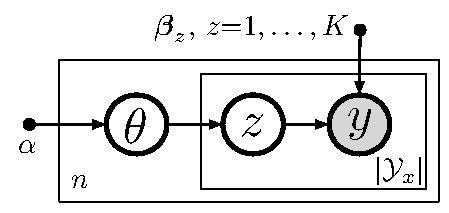
\includegraphics[width=0.6\fullwidth]{lda.pdf}}\\
\caption{潜在的ディリクレ配分法 (LDA) のモデル\cite{jmlr:03:05}}
\label{fig:lda}
\end{figure}

pLSAでは新規の利用者に対応できない問題があったが,これにベイズの枠組に拡張することで対応する\textbf{潜在的ディリクレ配分法 (latent Dirichlet allocation; LDA)}~\cite{jmlr:03:05}がある.
\index{LDA}
式\eqref{eq:origplsamodel}のpLSAモデルでは,最初に既知の利用者を$\calX$の中から$\pb{x}$に従って選択し,その利用者の嗜好パターンの分布$\pb{z|x}$に基づいて選んだ嗜好パターンに基づいてアイテムを選択する.
そのため,訓練データに表れない利用者については,その嗜好パターンが不明であり,pLSAでは対応できない.
そこで,嗜好パターン$\bftheta$自体をディリクレ分布に従って生成するように拡張することで,新規利用者に対応できるようにしたのがこのLDAである.
このLDAでは,訓練データ中の利用者$x$は,
しかし,変分ベイズやMCMCを用いた近似計算が必要になり,pLSAより計算量は増大する.
このLDAと類似したモデルとして\cite{icml:04:07}などもある.
%@@@ LDAについてもっと詳しく

%@@@ www:07:01 のMapReduceを用いた実装について

\section{時系列モデル}
\label{sec:timeseries}
\index{時系列}\index{time series}

時間に伴う変化を嗜好の予測に利用する方法を紹介する.
\ref{sec:getprefother}節で述べたように,標本利用者の時間順の行動や評価の履歴情報を,利用者DBに蓄積している場合がある.
この情報から,利用者の行動の時間的推移を表すモデルを構築し,活動利用者の現在にいたる行動や評価とこのモデルから,嗜好を予測する手法を紹介する.

\subsection{基本的な時系列モデル}

レンタルビデオ店で,先々週はあるドラマの第1話を,先週はこのドラマの第2話を借りていった顧客がいたとする.
このとき,今週はこのドラマの第3話を借りるだろうことは容易に予測できる.
この購入履歴に基づくモデルを利用した文献\cite{nips:03:03}の方法を紹介する.
利用者が$t$回目に購入したアイテムを$y^{(t)}$で表すと,購入履歴の系列は$\ang{Y^{(t)}}=\ang{y^{(1)},y^{(2)},\dotsc,y^{(t)}}$となる.
例えば,上記の連続ドラマの例であれば$y^{(1)}$〜$y^{(3)}$は,それぞれドラマの第1〜3回に相当する.
この購入履歴が与えられたときの,次に購入するアイテムの条件付確率$\pb{y^{(t+1)}|\ang{Y^{(t)}}}$を求めておき,この確率を最大にするアイテムを推薦する手法を考える.
これは,標本利用者の購入履歴を数え上げれば原理的には計算可能である.
しかし,\ref{sec:rsyslimit}節で述べたようにデータが疎であるので,いたるところで確率が$0$となり,実際にはこの方法では計算できない.
このような場合には,$K$回前までの状態,すなわち購入アイテムに基づく$K$重マルコフモデルを用いることが多い.
しかし,推薦の場合にはかなり過去の情報も次の状態に影響するため,単純にこのモデルを適用してもあまり有効ではない.

そこで,自然言語処理の言語モデルでよく利用される\textbf{最大エントロピーモデル (maximum entropy model; MaxEnt model)}を導入する.
\index{最大エントロピーモデル}\index{maximum entropy model}
\begin{equation}
\pb{y^{(t+1)}|\ang{Y^{(t)}}}=
\frac{1}{Z}
\exp\bra{\sum_{k=1}^K\lambda_k f_k\prn{y^{(t+1)},\ang{Y^{(t)}}}}
\label{eq:maxent}
\end{equation}
ただし,$Z$は正規化定数,$\lambda_k$は重みパラメータである.
ここで\term{素性関数}{feature function} $f_k\prn{y^{(t+1)},\ang{Y^{(t)}}}$が重要になる.
素性関数は購入履歴$\ang{Y^{(t)}}$にある特徴があるとき,次回に購入するアイテムがある特定のものになるなら$1$をとり,それ以外
では$0$となるような関数である.
例えば,上記のドラマの場合,購入履歴にドラマの第2回が含まれていて,次回購入がドラマの第3回なら$1$になる関数である.
このような素性関数をtriggerと呼ぶ.
このtriggerには,購入履歴中にアイテム$y$があるときに,次回にアイテム$y'$を購入する確率
$\pb{y^{(t+1)}=y'|y\in \ang{Y^{(t)}}}$と$\pb{y^{(t+1)}=y'}$との差が大きなものを選ぶ.
こうして素数関数を選択すれば,式\eqref{eq:maxent}のモデルのパラメータ$\lambda_k$は最大エントロピー原理\cite{jb:031:00}に基づいて推定できる.
素性関数には,trigger以外にも,いろいろなものが利用できる.
次に購入するアイテムが,$s\in{0,1,2,\dotsc}$個前に購入したアイテムに依存して決まるgapマルコフモデルを素性として利用する方法\cite{trieice:07:01}.
利用者自身の個人属性情報を考慮するのも有効であろう.
系列パターンマイニング\cite{eb:044:00,icde:01:02}などと組み合わせれば,triggerよりも複雑なパターンも素性関数として利用できるだろう.

\subsection{マルコフ決定過程モデル}

\begin{figure}
\centering
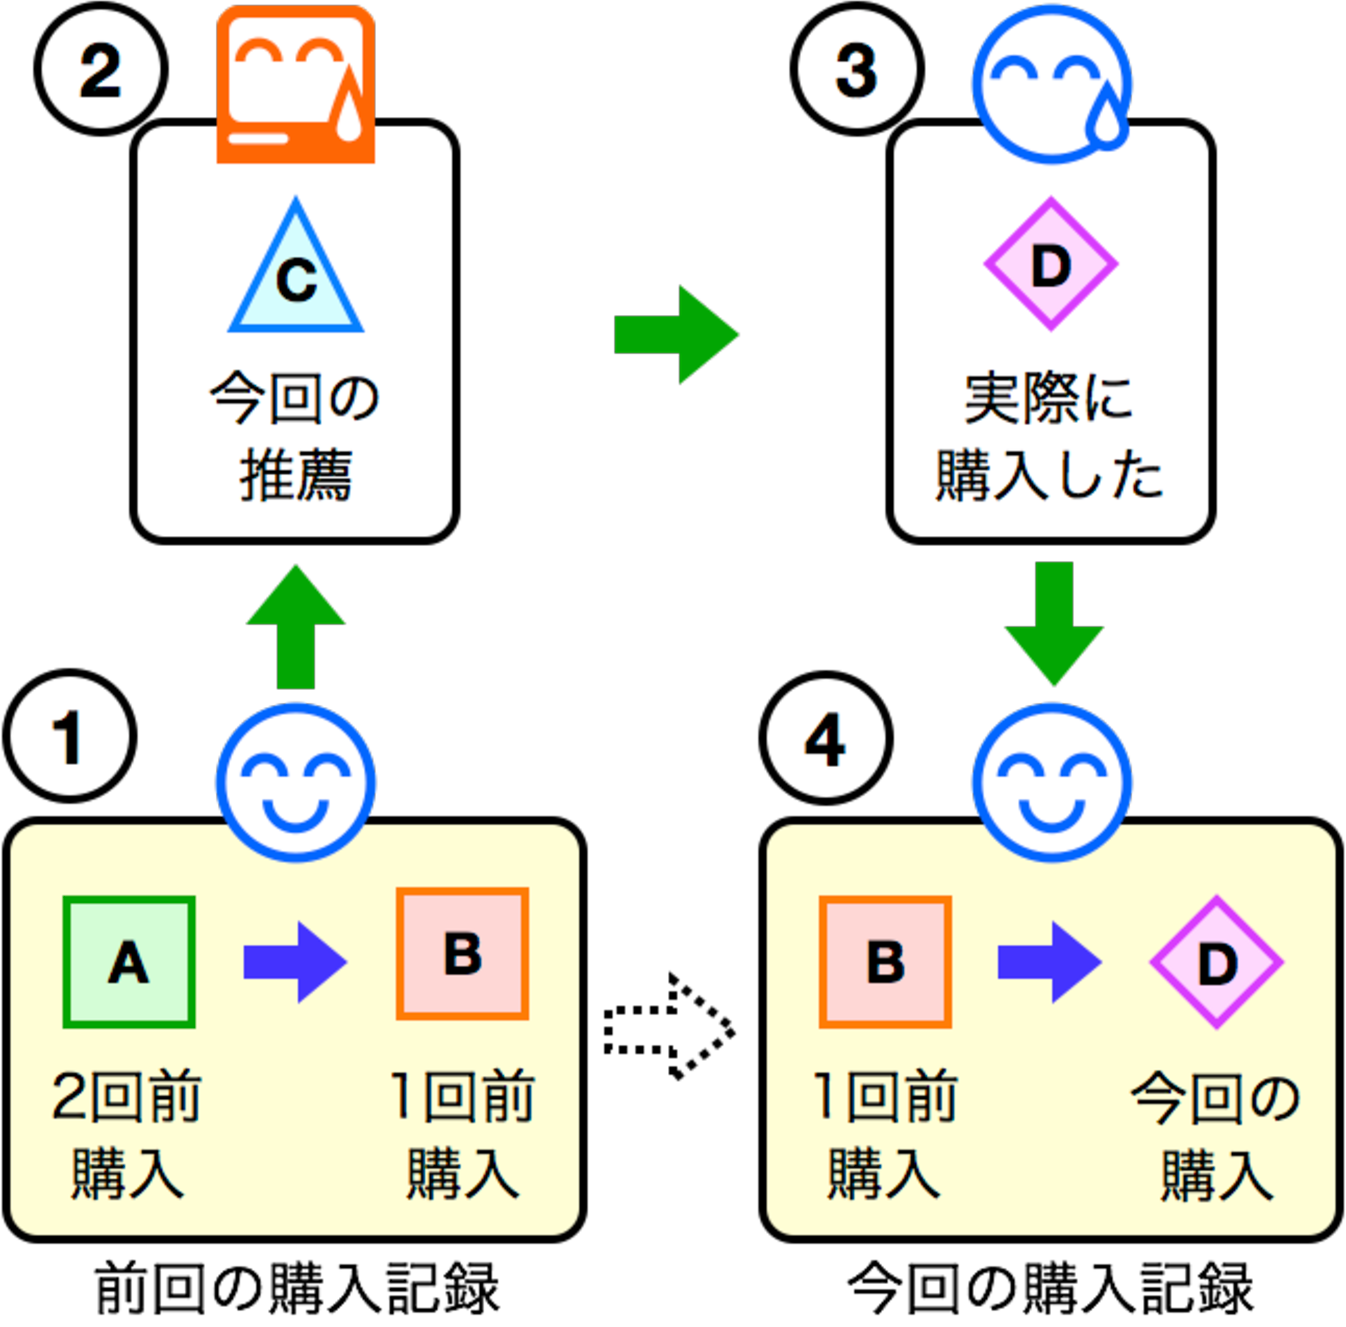
\includegraphics[width=0.6\fullwidth]{mdp.pdf}
\caption{マルコフ決定過程によるモデル}
\label{fig:mdpmodel}
\end{figure}

前節のモデルでは,過去の履歴に基づいて,次に利用者が選択する確率が最も高いアイテムを推薦する.
だが,推薦がなければそのアイテムを買ったかもしれないが,推薦の影響によってそのアイテムを選ばないという場合もある.
加えて,1年間全体で見て,選択したアイテムの価格の総和を最大化するとか,選択したアイテムへの利用者の評価の総和を最大にするような推薦をしたいとする.
これらの目的を達成するため,\term{マルコフ決定過程}{Markov decision process}を使う手法が提案されている\cite{uai:02:02,jmlr:05:03}.

マルコフ決定過程の前に\term{マルコフ過程}{Markov process}について述べる.
この過程では,次に選択するアイテム$y^{(t+1)}$は,直前の$K$個のアイテム系列$\ang{Y^{(t)}}=\ang{y^{(t-K+1)},\dotsc,y^{(t)}}$に依存する.
このアイテム系列で状態を表し,状態の遷移確率は$\mathrm{tr}_\mathrm{MC}(\langle Y^{(t)}\rangle,\langle Y^{(t+1)}\rangle)$と記す.
この確率は,十分なデータがあれば,利用者の購買履歴を数え上げれば計算できる.
しかし,データは疎なので,文献\cite{uai:02:02,jmlr:05:03}ではskippingや,アイテムのクラスタリングなどの手法を用いて対処している.

次にマルコフ決定過程を図\ref{fig:mdpmodel}を用いて説明する.
図中\ajMaru{1}は現在の状態$\ang{Y^{(t)}}=\ang{y^{(t-1)}=A,y^{(t)}=B}$で,この時刻$t$にアイテムDを購入
して,図中\ajMaru{4}の次の状態$\ang{Y^{(t+1)}}=\ang{y^{(t)}=B,y^{(t+1)}=D}$に移る.
ここで,単に$\ang{Y^{(t)}}$のみに依存して$\ang{Y^{(t+1)}}$が決まる(図の点線矢印)ならマルコフ過程である.
それとは異なり,マルコフ決定過程では,状態$\ang{Y^{(t)}}$で行う推薦という行動(action)を明示的に考慮する.
これにより,推薦という行動によって,利用者の選択が変わることをモデル化できる.
この時刻$t$での行動$A^{(t)}$は図中\ajMaru{2}にあたり,アイテム$C$を推薦した.
利用者は$\ang{Y^{(t)}}$と$A^{(t)}$に依存して,アイテム$y^{(t+1)}$を選択し,次の状態$\ang{Y^{(t+1)}}$に遷移する.
図の例では,推薦を受け入れず利用者は\ajMaru{3}でアイテムDを購入したので,遷移した状態は\textcircled{\small 4}の$\ang{Y^{(t+1)}}=\ang{B,D}$となった.
この状態遷移を$\prn{\ang{Y^{(t)}},A^{(t)},\ang{Y^{(t+1)}}}$と,この遷移確率を$\Pr_\mathrm{MDP}\bra{\ang{Y^{(t)}},A^{(t)},\ang{Y^{(t+1)}}}$と記す.
また,状態$\ang{Y^{(t)}}$で行動$A^{(t)}$を決定する手続きを方策 (policy) と呼ぶ.
さらに,図の\ajMaru{3}にてアイテムDを選択したが,これに依存して報酬 (reward) が発生する.
この報酬は,アイテムへの代金や,利用者のアイテムへの評価値などである.
報酬の導入により,個別の推薦ごとの効用を最大化するのではなく,複数の推薦を含む長期間の効用の最大化を考慮できるようになる.
この報酬を最大化するような政策を決める学習問題は\term{強化学習}{reinforcement learning}\cite{eb:058:00,jb:019:00}と呼ばれる.
既存の強化学習の方法を用いて,適切な政策が獲得できれば,推薦は政策に従うことで実行可能になる.
ただし,データが疎である問題に対処するため,マルコフ決定過程の遷移確率$\Pr_\mathrm{MDP}\bra{\ang{Y^{(t)}}, A^{(t)},\ang{Y^{(t+1)}}}$を,マルコフ過程の遷移確率$\Pr_\mathrm{MC}\bra{\ang{Y^{(t)}}, \ang{Y^{(t+1)}}}$によって初期
化するなどのヒューリスティックを用いている.

\subsection{定期購入サービス}

時系列を扱う手法の最後に\term{定期購入}{subscription}というサービスを対象とした手法を紹介する\cite{kdd:06:02}.
定期購入サービスとは音楽配信などのサービスの販売形式の一つで,契約すると,解約するまでの期間,任意の曲を任意の回数試聴できる.
そのため,個々の購入での満足ではなく,サービス全体への顧客満足度を向上させて,解約を防ぐことが目標になる.
上記の強化学習の枠組みでは,各購入行動ごとに時間$t$が経過する.
一方,サブスクリプションでは,各行動が何回目であるかを示す$t$に加え,実時間と共に推移する契約期間$T$もモデル化する必要がある.

利用者$x$に$t$回目にアイテム$y^{(t)}$を推薦したとき,現在の契約期間中に解約しない事象$e$が生じる確率を最大化するようなアイテムを推薦する.
\[
 \hat{y}^{(t)}=\arg\max_{y^{(t)}\in\calY}\pb{e|x,y^{(t)}}
\]
推薦の結果,実際に購入したアイテムを${y'}^{(t)}$で表し,この確率を次のように分解する.
\[
\pb{e|x,y^{(t)}}=
\sum_{{y'}^{(t)}\in\calY}
\pb{e|x,{y'}^{(t)}} \pb{{y'}^{(t)}|x,y^{(t)}}
\]
利用者$x$がアイテム${y'}^{(t)}$を選択したとき解約しない確率が$\pb{e|x,{y'}^{(t)}}$で,$y^{(t)}$を推薦したときに${y'}^{(t)}$を選
択する確率が$\pb{{y'}^{(t)}|x,y^{(t)}}$である.
前者の確率は,\term{ハザード関数}{hazard function} $h\prn{T|\ang{Y^{(t)}}}$で表す.
これは購入履歴が$\ang{Y^{(t)}}=\ang{y^{(1)},\dotsc,y^{(t)}}$である利用者のうち,期間$T$まで契約を継続し,かつ,この時点で契約をやめる割合を示す.
この関数は生存時間分析 (survival analysis) の\term{Cox比例ハザードモデル}{Cox proportional hazards model}でモデル化する.
$\ang{Y^{(t-1)}}$のあとに${y'}^{(t)}$を購入した系列を$\ang{Y^{(t-1)},{y'}^{(t)}}$で表すと$\pb{e|x,{y'}^{(t)}}$は,適当な仮定の下,次式となる.
\[
\pb{e|x,{y'}^{(t)}}=
\frac{h(T|\ang{Y^{(t-1)}})}{h\prn{T|\ang{Y^{(t-1)}}}+h\prn{T|\ang{Y^{(t-1)},{y'}^{(t)}}}}
\]
一方の$\pb{{y'}^{(t)}|x,y^{(t)}}$は,アイテムを推薦することにより選択確率が定数倍されると仮定して,利用者$x$の選択確率$\pb{{y'}^{(t)}|x}$から求める.
この$\pb{{y'}^{(t)}|x}$は,購入履歴に基づく素性関数を用いた最大エントロピーモデルでモデル化する.
\index{最大エントロピーモデル}\index{maximum entropy model}
このようにモデル化すれば,あとは購入履歴からパラメータを学習すればよい.
